Poslední kapitola této diplomové práce popisuje testování funkcionality nástroje pro podporu automatické správy virtualizačního
kontejneru Solaris Zones. Zaměřuje se především na testování
hlavních scénářů použití nástroje a~zkoumá jeho chování. Na začátku této kapitoly je definováno prostředí, ve kterém byly
testy prováděny. Následuje série testů, které zkoumají funkcionalitu nástroje v~konkrétních případech použití. Kapitola je zakončena
měřením, které zkoumá dobu trvání některých funkcí nástroje.
\section{Definice testovacího prostředí}
\label{chapter:testing:environment}
Pro účely testování výše zmíněného nástroje bylo nutné vytvořit prostředí odpovídající jeho cílové platformě. Toto prostředí
obsahuje několik virtualizačních serverů s~operačním systémem Solaris, který bude poskytovat své prostředky neglobálním zónám.
Tyto servery jsou propojeny počítačovou sítí, pomocí které je lze ovládat. Tato infrastruktura byla virtualizovaně vytvořena na 
fyzickém systému s~následujícími parametry:
\begin{itemize}
 \item procesor Intel(R) Xeon(R) CPU E3-1230 v3 (3.30Ghz),
 \item RAM 16GB,
 \item operační systém Windows 10 (64-bit).
\end{itemize}
Virtualizace architektury byla docílena pomocí virtualizační technologie Virtualbox, která umožňuje spouštění virtuálních 
počítačů v~rámci jiného operačního systému. Pomocí této technologie byly vytvořeny tři virtuální stroje s~operačním systémem
Solaris ve verzi 11.3. Tyto stroje byly propojeny pomocí virtuální počítačové sítě a~nakonfigurovány tak, aby se na ně dalo 
připojovat pomocí SSH. Dále byly jednotlivým strojů přiřazena doménová jména \textit{shost}, \textit{shost1} a~\textit{shost2}.
Tato doménová jména byla nakonfigurována pomocí souboru \textit{/etc/hosts} na všech zmíněných virtuálních počítačích. Toto
nastavení umožňuje používat specifikovaná doménová jména místo IP adres a~zjednoduší tak identifikaci strojů v~testovacích
ukázkách. 

Jelikož provozování virtualizační technologie Solaris Zones vyžaduje nemalé množství výpočetních prostředků, bylo nutné
dostupné prostředky fyzického systému rozdělit mezi virtuální stroje. Z~tohoto důvodu byly každému virtuálnímu počítači
přiřazeny následující výpočetní prostředky:
\begin{itemize}
 \item jedno jádro fyzického procesoru,
 \item RAM 3 GB,
 \item virtuální disk 50 GB (HDD).
\end{itemize}

Na virtuální počítač s~doménovým jménem \textit{shost} byl nainstalován interpret programovacího jazyka Ruby ve verzi 2.4.2.
Dále byla na stejný počítač nainstalována Java ve verzi 1.8.0\_60 a~následně druhý interpret programovacího jazyka Ruby
tentokrát ve verzi 2.3.3 a~implementaci JRuby. Pokud není uvedeno jinak, testovaný nástroj byl vždy spouštěn z~virtuálního
počítače s~doménovým jménem \textit{shost}.

Posledním učiněným krokem byla konfigurace uživatele \textit{zadmin}, který má práva na vykonávání příkazů nutných ke správnému
chodu implementovaného nástroje. Tyto nástroje byly vyjmenovány v~kapitole \ref{chapter:design:architecture:szones}. Uživatel 
byl pomocí nástroje RBAC vytvořen a~nakonfigurován na všech vytvořených virtuálních počítačích.
\section{Testování scénářů použití}
\label{chapter:testing:scenario}
V~následujících kapitolách je popsáno akceptační testování hlavních scénářů použití nástroje pro podporu automatické správy
Solaris Zones. Pro testování aplikace bylo vždy použito popsané prostředí, pokud není uvedeno jinak. Na~začátku každého scénáře
je stanoven cíl, který by uživatel mohl chtít pomocí implementovaného nástroje dosáhnout. Následně je popsán stav prostředí, ve~kterém
se systém nacházel před provedením konkrétní akce. Dále byl proveden korespondující příkaz v~uživatelském rozhraní nástroje,
který má splnit stanovený cíl. Výsledek tohoto kroku je ověřen pomocí systémových příkazů a~v~závěru scénáře je rozhodnuto, zda bylo
dosaženo stanoveného cíle.
\subsection{Vytvoření neglobálních zón ze šablony}
\label{chapter:testing:scenario:deploy_template}
Pro komplexní otestování funkcionality implementovaného nástroje byl zvolen scénář vytvoření několika neglobálních zón pomocí
šablony. Hlavní důvod pro~výběr tohoto scénáře je, že se do tohoto procesu zapojují téměř všechny části nástroje.

Cílem tohoto scénáře je vytvoření několika neglobálních zón na~různých hostech v~rámci dané infrastruktury. Jako zdroj byla 
použita šablona popsaná v~kapitole \ref{chapter:implementation:szones:template}. Ze~šablony byly vybrány některé důležité 
vlastnosti, které mají vytvořené zóny mít. Typ zóny byl stanoven jako \textit{solaris} s~exkluzivní IP adresou. Dále má 
nainstalovaná zóna obsahovat softwarové balíky pro správu zdrojového kódu. Tyto balíky obsahují nástroje \verb|hg|
a~\verb|git|. Šablona také definuje počáteční heslo uživatele \textit{root} a~nastavuje typ tohoto uživatelského účtu na roli.
Vedle uživatele \textit{root} je v~šabloně definován počáteční systémový uživatel, který má být zároveň systémovým administrátorem.
Vytvářené neglobální zóny mají mít jedno síťové rozhraní se jménem \textit{net0}, které bude konfigurováno automaticky pomocí
DHCP. Takto definovaná šablona je uložena na severu s~doménovým jménem \textit{shost}.

Příkaz pro vytvoření čtyř zón pomocí uživatelského rozhraní nástroje je v~ukázce kódu \ref{code:test:deployment} na první řádce.
Tento příkaz říká, že mají být vytvořeny zóny \textit{zdev} a~\textit{zdev1} na lokálním serveru a~zóna \textit{zdev} na vzdálených
serverech \textit{shost1} a~\textit{shost2}. Jako parametr \textit{specification} je udána cesta k~šabloně s~výše popsanými 
vlastnostmi. Dále byl příkazu předán parametr \textit{boot}, který má rovnou spustit vytvořené zóny.

Z~konce standardního výstupu nástroje v~ukázce výpisu programu \ref{code:test:deployment} je patrné, že vytvoření všech neglobálních zón
proběhlo v~pořádku. Jelikož se pro~vytváření zón používá stejná rutina a~stejná šablona, musí mít všechny stejné parametry.
Pro otestování korektnosti práce nástroje byla použita neglobální zóna \textit{zdev} na vzdáleném serveru \textit{shost2}.
Korektní vytvoření a~spuštění zóny bylo ověřeno pomocí nástroje \verb|zlogin(1)|, který umožňuje připojení k~příkazové řádce dané
zóny. Úspěšné přihlášení v~ukázce výpisu programu \ref{code:test:deployment:result} signalizovalo hned několik věcí. Za prvé se zdárně
podařilo vytvořit a~spustit danou zónu a~za druhé byly správně nakonfigurovány uživatelské systémové služby pomocí atributů ze šablony.
Dále je z~ukázky výpisu programu \ref{code:test:deployment:result} patrné, že došlo k~vytvoření síťového adaptérů \textit{net0} a~jeho automatické
konfigurace pomocí služby DHCP. Přítomnost softwarových
balíků byla otestována pomocí jejich rozhraní na příkazové řádce, jak je vidět v~ukázce výpisu programu \ref{code:test:deployment:result}.
Posledním kritériem úspěchu bylo správné nakonfigurování počátečního systémového uživatele. Jméno a~heslo bylo ověřeno již
při přihlašování do zóny. Zbývalo tedy ověřit, zda uživatel má práva systémového administrátora, což bylo provedeno pomocí
příkazu \verb|profile|. Výpis programu na ukázce \ref{code:test:deployment:result} je zkrácený, ale obsahuje profil \textit{System Administrator}.

Pomocí výše zmíněných testů bylo ověřeno, že se daná zóna vytvořila, spustila a~že měla vlastnosti specifikované v~použité šabloně.
Stejným způsobem byly ověřeny i ostatní vytvářené zóny. Jelikož tyto zóny vykazovaly stejné chování a~vlastnosti, byl tento
test uzavřen a~považován za splněný.
\subsection{Využití uživatelského žurnálu}
\label{chapter:testing:scenario:journal}
Dalším využitím implementovaného nástroje může být využití uživatelského žurnálu. Cílem následujícího scénáře je kontrola 
funkcionality uživatelského žurnálu a~jeho schopnosti informovat uživatele o~změnách neglobálních zón v~rámci infrastruktury.
K~tomuto účelu byl využitý stav, ve kterém se systém nacházel po testování předchozího scénáře. Součástí předchozího scénáře
bylo vytvoření čtyř zón pomocí implementovaného
nástroje. Před tímto vytvořením se v~systému nenacházely žádné jiné neglobální zóny. V~tomto stavu by měl uživatelský žurnál 
obsahovat čtyři zóny ve stavu \textit{running}. Jak je vidět z~výpisu programu \ref{code:test:journal}, součástí uživatelského
žurnálu byly opravdu čtyři zóny ve stavu \textit{running} a~výpis neobsahoval žádné jiné nesledované neglobální zóny.
Toto zjištění indikovalo, že nástroj opravdu aktualizuje uživatelský nástroj po provedení akcí.

Následně byla simulována situace, kdy jiný uživatel změní konkrétním způsobem stav sledované zóny. Konkrétně byla bez pomoci 
implementovaného nástroje přeinstalována zóna \textit{zdev} na vzdáleném serveru \textit{shost2} a~její stav byl změněn z~původního
\textit{running} na \textit{installed}. Dále byla vytvořena nová zóna \textit{zdev-clone} na stejném vzdáleném počítači. V~tomto
případě by měl uživatel při dalším vypsání uživatelského žurnálu zjistit, že se změnil stav a~diskový obraz dané zóny 
\textit{zdev}. Součástí výpisu by měla být i informace o~nově vytvořené zóny v~rámci infrastruktury. Z~ukázky výpisu programu 
\ref{code:test:journal:change} je vidět, že uživatelský žurnál opravdu informuje uživatele o~změně sledované zóny a~na~konci
výpisu je zobrazena informace o~nově vytvořené zóně. Ostatní sledované zóny byly z~výpisu vynechány.

Pomocí implementovaného nástroje může uživatel neglobální zóny vytvářet, mazat nebo měnit jejich stav. Jak bylo zjištěno
na začátku této kapitoly, nástroj aktualizuje konkrétní záznam v~uživatelském žurnálu, pokud danou zónu vytváří. Podobným
způsobem bylo ověřeno, že uživatelský žurnál je aktualizován i při mazání a~změně stavu zóny. Dále tento scénář ověřil funkcionalitu
žurnálu, která má informovat uživatele v~případě, kdy dojde ke změně stavu sledované zóny nebo vytvoření nové zóny v~rámci
infrastruktury. Z~výše uvedených důvodů bylo testování využití uživatelského žurnálu označeno za~úspěšné.
\subsection{Migrace neglobálních zón}
\label{chapter:testing:scenario:migration}
V~rámci testování nástroje pro podporu automatické správy virtualizačního kontejneru Solaris Zones byl otestován scénář, který
zahrnuje migraci neglobálních zón mezi dvěma hosty. Jelikož nástroj umožňuje migraci zón jak z~lokálního tak ze vzdálených serverů,
bylo nutné vybrat komplexní scénář pokrývající tyto možnosti. Pro komplexní ověření této funkcionality nástroje bylo na hostech 
\textit{shost} a~\textit{shost1} vytvořeno několik neglobálních zón, které byly migrovány na cílový vzdálený server \textit{shost2}. 
Pro účely tohoto scénáře byla využita technika přímého přenosu souborového systému, kterou implementovaný nástroj poskytuje.

Cílem tohoto scénáře je přesunutí neglobálních zón ze zdrojových serverů na cílový server. Na obou zdrojových serverech se na
začátku testování nacházely následující neglobální zóny:
\begin{itemize}
 \item \textit{zmigr:localhost},
 \item \textit{zmigr1:localhost},
 \item \textit{zmigr2:shost1},
 \item \textit{zmigr3:shost1}.
\end{itemize}
Po provedení migrace by se tyto zóny měly nacházet na cílovém serveru \textit{shost2} a~na zdrojových serverech by se neměly
nacházet žádné neglobální zóny. Uživatelský žurnál zobrazený ve výpisu programu \ref{code:test:migration:before} potvrzoval
stav před provedením migrace.
 
Pro migraci neglobálních zón slouží příkaz \verb|migrate|, který je možné využívat skrze uživatelské rozhraní implementovaného
nástroje. Právě tento příkaz byl použit pro testování tohoto scénáře a~ve výpisu programu \ref{code:test:migration} je možné pozorovat jeho
výstup. Jak výstupu patrné, všechny zóny byly podle nástroje úspěšně přesunuty na cílový server \textit{shost2}. 
Pro ověření funkcionality bylo nutné ověřit, zda se zóny opravdu nachází na cílovém serveru, zda jsou zóny smazány
ze zdrojových serverů a~také zda nástroj aktualizoval uživatelský žurnál.

Pomocí nástroje \verb|zoneadm(1)| a~příkazu \verb|list| bylo ověřeno, že na vzdáleném serveru se opravdu nachází přesunuté zóny.
Na zdrojových serverech byl spuštěn stejný příkaz pro ověření, že se na nich nenachází žádné neglobální zóny. Výstup těchto kroků
je zobrazen ve výpisu programu \ref{code:test:migration:list}. Těmito kroky bylo ověřeno, že nástroj správně pracuje se zónami a~umožňuje
jejich přesun v~rámci jednotlivých serverů infrastruktury. Dále bylo nutné ověřit, zda nástroj správně aktualizuje konkrétní záznamy
v~uživatelském žurnálu. Stav ve výpisu programu \ref{code:test:migration:before} by se měl změnit tak, že přesouvané zóny budou
zobrazeny pod~hostem \textit{shost2}. Tato skutečnost je potvrzena výpisem programu \ref{code:test:migration:after}, který ukazuje očekávaný
výstup uživatelského žurnálu.

Výše popsaný testovací scénář dokazuje správné chování implementovaného nástroje v~případě, kdy uživatel využívá administračních
funkcí pro migraci zón. Test potvrzuje, že uživatel je schopný přesouvat neglobální zóny z~lokálního i ze vzdáleného serveru
na vzdálený cílový server. Migrace je provedena najednou a~nástroj po jejím úspěšném provedení adekvátně aktualizuje uživatelský žurnál.
Z~výše popsaných důvodů bylo testování migračního scénáře označeno za úspěšné.
\subsection{Záloha a~obnova zón}
\label{chapter:testing:scenario:backup_recovery}
Dalším testovaným scénářem bylo vytvoření zálohy a~následná obnova. Jelikož se jedná o~dvě samostatné funkce nástroje, byl
tento test rozdělený do~dvou samostatných scénářů. V~prvním scénáři použití bylo otestováno vytvoření zálohy několika zón. 
Následující scénář potom využil vytvořené zálohy k~obnovení stejných zón.
\subsubsection{Záloha neglobálních zón}
\label{chapter:testing:scenario:backup_recovery:backup}
Cílem tohoto scénáře bylo ověření funkcionality nástroje ve vytváření záloh neglobálních zón. Při procesu vytváření zálohy má
nástroj za úkol vytvořit archiv souborového systému zálohované zóny. Nástroj umožňuje vytvoření zálohy pomocí dvou typů archivů.
V~případě tohoto scénáře byl použit archiv typu UAR. Dále nástroj umožňuje specifikovat vzdálený server a~cestu, kam má být
záloha uložena. Pomocí tohoto scénáře bylo ověřeno, zda nástroj tuto funkcionalitu opravdu umožňuje. Pro kompletní ověření
funkcionality bude sloužit následující scénář, který z~vytvořených záloh bude zóny obnovovat. Pro účely tohoto scénáře byly
v~infrastruktuře vytvořeny následující zóny:
\begin{itemize}
 \item \textit{zback:shost2},
 \item \textit{zback1:shost2},
 \item \textit{zback2:shost1},
 \item \textit{zback3:shost1}.
\end{itemize}
Na lokálním serveru \textit{shost} byl vytvořen zálohovací adresář \textit{/zonepool/backup}, ve kterém se před zahájením
testu nenacházely žádné soubory.

Nástroj pro zálohování zón nabízí příkaz \verb|backup|, který je možný využít v~uživatelském rozhraní. Pomocí tohoto příkazu byla
spuštěna záloha výše zmíněných zón. Výstup tohoto příkazu je zobrazen ve výpisu programu \ref{code:test:backup} a~ukazuje, že záloha
zón proběhla úspěšně. Zálohy by se podle výstupu programu měly nacházet ve~složce \textit{/zonepool/backup} na lokálním serveru.

Pomocí standardního nástroje \verb|ls(1)| bylo ověřeno, že se zálohy opravdu vytvořily a~že se nacházely v~určeném adresáři na
lokálním serveru. Tento testovací scénář potvrzuje, že nástroj je schopný najednou vytvářet zálohy více neglobálních zón
různě umístěných v~infrastruktuře serverů. Dále potvrzuje, že nástroj umí stáhnout zálohy do konkrétního adresáře na předem
určeném serveru. Z~výše zmíněných důvodů bylo testování vytváření zálohy neglobálních zón úspěšné.
\subsubsection{Obnova neglobálních zón}
\label{chapter:testing:scenario:backup_recovery:recovery}
Posledním testovaným scénářem použití nástroje byla obnova neglobálních zón z~archivu. Cílem testování tohoto scénáře bylo 
ověření, zda nástroj umí obnovit (vytvořit) neglobální zóny pomocí dříve vytvořených záloh. Jako zdrojové archivy byly použity
zálohy vytvořené během předchozího testování. Pro simulaci ztráty dat byly všechny zóny z~minulého testování odstraněny
a~zachovány byly pouze jejich archivy ve složce \textit{/zonepool/backup} na lokálním serveru. Výsledkem obnovy by mělo být
vytvoření všech zón ze zálohy a~jejich umístění na původní servery. 

Ve složce \textit{/zonepool/backup} se na začátku testování nacházely čtyři archivy typu UAR, které obsahovaly diskové obrazy
a~konfigurace jednotlivých zón. Nástroj pro podporu automatické správy Solaris Zones poskytuje funkcionalitu pro obnovu zón skrze
příkaz \verb|recovery|. Pomocí tohoto příkazu byla spuštěna obnova z~výše zmíněných archivů. Tento proces je vyznačen ve výpisu
programu \ref{code:test:recovery}, kde je vidět i výstup tohoto příkazu. Z~příkazu je patrné, že pořadí specifikace identifikátorů
zón musí odpovídat pořadí zadaných archivů. Pokud by toto pořadí nesouhlasilo, došlo by k~výměně diskových obrazů daných
zón. Podle výstupu nástroje proběhla obnova zón v~pořádku a~zóny by měly být nainstalovány na své původní hosty.

Stejně jako v~ostatních případech vytváření zón bylo pomocí nástroje \verb|zoneadm(1)| a~příkazu \verb|list| ověřeno, že se
obnovené zóny opravdu vytvořily na daných vzdálených serverech. Testování tohoto scénáře potvrdilo, že nástroj umí obnovit
neglobální zóny ze sady záloh. Tyto zálohy musí mít definovaný tvar.
V~případě tohoto scénáře se jednalo o~zálohy typu UAR, které byly vytvořeny v~rámci předchozího testování. Z~tohoto důvodu je možné
označit testování scénáře pro obnovu zón za úspěšné.
\section{Měření}
\label{chapter:measurement}
V~rámci testování nástroje pro podporu automatické správy virtualizačního kontejneru Solaris Zones bylo provedeno měření doby
běhu dvou hlavních administrátorských rutin. Konkrétně se jednalo o~měření doby běhu vytváření neglobálních zón a~jejich migrace
v~rámci popsané infrastruktury. V~obou případech byla sledována doba běhu dané rutiny v~závislosti na počtu vytvářených nebo
přenášených zón. Tato měření byla prováděna pro několik technik vytváření a migrace neglobálních zón. Podrobně jsou obě měření
popsána v~následujících kapitolách. Jelikož vytváření a migrace většího počtu zón na~jednom fyzickém stroji potřebuje větší 
výpočetní nároky, byly pro tato měření použity pouze virtuální stroje \textit{shost} a \textit{shost1}. Oběma strojům byly
přiřazeny čtyři procesorová jádra. Kromě výše zmíněné změny bylo použito prostředí popsané v~kapitole \ref{chapter:testing:environment}.
\subsection{Techniky vytváření zón}
\label{chapter:measurement:creation}
Prvním objektem měření bylo sledování doby běhu nástroje při vytváření zón v~závislosti na jejich počtu a technice vytváření. Cílovým
serverem instalace byl lokální server \textit{shost}. Pro toto měření byly použity následující techniky vytváření neglobálních zón:
\begin{itemize}
 \item klonování,
 \item instalace ze šablony,
 \item instalace ze vzdálené zóny.
\end{itemize}
Pro účely klonování byla na lokálním serveru \textit{shost} vytvořena instance šablony \textit{template\_z1}, která sloužila jako 
předloha pro klonování. Zdrojový souborový systém této zóny se v~průběhu měření opakovaně klonoval a zkoumala se doba běhu
v~závislosti na počtu vytvářených klonů. V~případě druhé techniky byla vytvořena šablona \textit{zweb}, která specifikuje neglobální
zónu. Její parametry nejsou pro měření podstatné. Tento typ instalace využívá online repozitář \cite{oracle:solaris:desing:pkg_repository}.
Z~tohoto důvodu je výsledná doba instalace ovlivněná kvalitou internetového připojení. Pro účely posledního typu instalace byla
na vzdáleném serveru \textit{shost1} vytvořena neglobální zóna \textit{z1}, která sloužila jako předloha pro instalaci zón. Ve
výsledné době běhu je tedy zahrnutý i přenos souborového systému ze vzdáleného serveru na lokální server.

Jak je patrné z~tabulce \ref{table:measuremet:creation_table}, měření bylo prováděno pro různé počty vytvářených zón. Maximální
hodnota byla stanovena na deset zón, protože pro větší počet zón by se výrazně projevovala omezení testovacího prostředí. Pro každou
kombinaci parametrů bylo měření několikrát opakováno a~výsledek zprůměrován. Přesné hodnoty naměřených časů je možné pozorovat v~tabulce
\ref{table:measuremet:creation_table}. Výsledky jsou také graficky znázorněny v~grafu \ref{graph:measuremet:creation_graph}.
\begin{table}[b]
  \centering
  \caption{Doba běhu vytváření zón v~závislosti na jejich počtu a použité technice}
  \begin{tabular}{ l | c c c c c}
   Počet zón & 1 & 2 & 4 & 8 & 10 \\ \hline
   Klonování [s] & 19.5 & 20.4 & 28.8 & 51.4 & 74.6 \\
   Šablona [s] & 378.6 & 543.2 & 897.4 & 1648.5 & 2154.1 \\
   Vzdálená zóna [s] & 136.5 & 189.7 & 320.1 & 668.6 & 819.5 \\
  \end{tabular}
  \label{table:measuremet:creation_table}
\end{table}

\begin{figure}
  \centering
  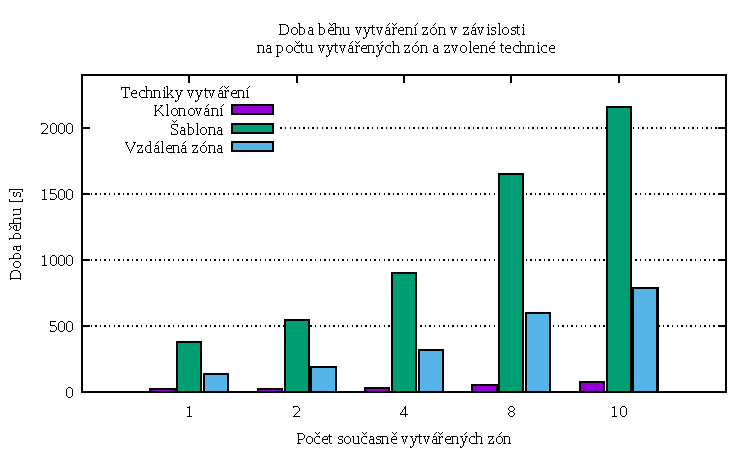
\includegraphics{assets/pdfs/measurement_creation.pdf}
  \caption{Doba běhu vytváření zón v~závislosti na jejich počtu a použité technice}
  \label{graph:measuremet:creation_graph}
\end{figure}

Z~provedeného měření je možné vypozorovat, že technika klonování zón je jednoznačně nejrychlejším způsobem vytváření zón. Časy
pro ostatní techniky nejsou tak malé, protože tyto způsoby instalace zahrnují vytváření archivů a přenosy velkých objemů dat
po síti. Velikost jedné neglobální zóny v~průběhu testování byla přibližně 1,5 GB. Pokud se má po síti přenášet několik takových
zón najednou, je nutné přenést opravdu velké množství dat. Jak je patrné z tabulky \ref{table:measuremet:creation_table}, měření
doby běhu instalace ze šablony bylo velmi závislé na propustnosti internetového připojení testovacího prostředí. Z tohoto důvodu
tato technika instalace v průběhu měření nevykazovala příliš dobré výsledky. Z~výše uvedeného měření plyne, že technika klonování
je v~rámci měřených způsobů nejrychlejší. Tato technika nešetří pouze čas instalace, ale také diskové místo.
\subsection{Techniky migrace zón}
\label{chapter:measurement:migration}
Druhé měření se zabývá různými technikami způsobu migrace zón a~měří dobu jejich trvání v~závislosti na počtu migrovaných zón.
Implementovaný nástroj umožňuje přenášet zóny mezi servery pomocí následujících technik:
\begin{itemize}
 \item přímá migrace,
 \item migrace pomocí ZFS archivu,
 \item migrace pomocí UAR archivu.
\end{itemize}
První technika využívá k~migraci přímo příkazy souborového systému ZFS a~umožňuje přenášet souborový systém bez nutnosti jeho dočasného
uložení. Migrace pomocí ZFS archivu je podobná přímé technice, ale v~průběhu migrace se zdrojový souborový systém uloží do archivu,
který je následně přenesen na cílový server. V~případě poslední techniky je použitý archiv typu UAR, který je standardním způsobem zálohování
v~operačním systému Solaris. I~tato technika vyžaduje dočasné uložení vytvořeného archivu. Provedené měření bylo zaměřeno
na porovnání doby trvání migrace v~závislosti na počtu migrovaných zón a~zvolené technice migrace.

Pro účel tohoto měření byly na lokálním serveru \textit{shost} vytvořeny neglobální zóny, které byly vždy přesouvány na vzdálený
server \textit{shost1}. Migrace byla několikrát opakována pro každou zmíněnou techniku a~počet migrovaných zón. Výsledná
doba běhu byla v~rámci opakování se stejnými hodnotami parametrů zprůměrována. Stejně jako v~minulém měření bylo přenášeno maximálně
deset neglobálních zón najednou. Naměřené hodnoty doby běhu pro různé počty migrovaných zón a~různé techniky migrace je možné
pozorovat v~tabulce \ref{table:measuremet:migration}. Graficky jsou tyto hodnoty znázorněny v~grafu \ref{graph:measuremet:migration}.
\begin{table}
  \centering
  \caption{Doba běhu migrace zón v~závislosti na použité metodě}
  \begin{tabular}{ l | c c c c c c}
   Počet zón & 1 & 2 & 4 & 8 & 10 &   \\ \hline
   Přímá technika [s] & 118.3 & 134.6 & 220.2 & 420.1 & 561.2 & \\
   Technika ZFS [s] & 133.5 & 196.1 & 291.5 & 580 & 723.7 & \\
   Technika UAR [s] & 167.8 & 449.7 & 729.5 & 1448.3 & 1793.6 & \\
  \end{tabular}
  \label{table:measuremet:migration}
\end{table}

\begin{figure}
  \centering
  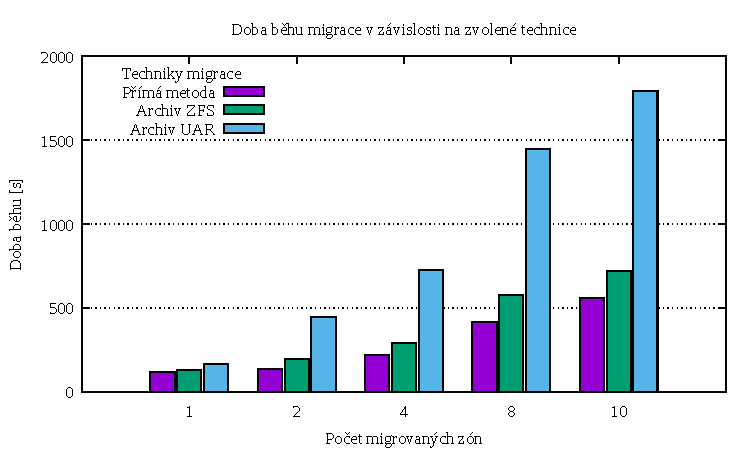
\includegraphics{assets/pdfs/measurement_migration.pdf}
  \caption{Doba běhu migrace zón v~závislosti na použité metodě}
  \label{graph:measuremet:migration}
\end{figure}

Z~měření je možné vypozorovat, že přímá technika migrace přenáší zóny nejrychleji. Tento výsledek se byl očekáván, jelikož tato technika nevyžaduje
dočasné ukládání přenášeného souborového systému. Technika využívající ZFS archivy je pomalejší. Důvodem je hlavně nutnost
dočasného uložení vytvořeného archivu na vzdáleném serveru. Výše zmíněné techniky jsou vykonávány paralelně pro všechny přenášené
zóny. V~případě techniky využívající archivy typu UAR tomu tak není. Jak je patrné z~tabulky \ref{table:measuremet:migration},
naměřené časy této techniky odpovídají sériovému provádění migrací. Tento fakt je způsobem nástrojem \verb|archiveadm(1)|, který
nemůže být současně používán více procesy v~rámci jednoho systému. Z~měření vyplynulo, že nejrychlejší technikou pro migraci zón je
přímá technika.
\section{Závěr testování}
\label{chapter:testing:scenario:conclusion}
V~rámci testování nástroje pro podporu automatické správy virtualizačního kontejneru Solaris Zones byly testovány hlavní scénáře
použití a změřena doba běhu některých funkcí nástroje. Popsaná měření dokazují, že implementovaný nástroj je schopen provádět administrátorské
rutiny pro větší množství neglobálních zón. S~rostoucím počtem těchto zón však roste i celková doba běhu programu. Z~měření je také patrné,
že některé funkce nástroje jsou v~určitých situacích výhodnější než jiné.

Všechny testované scénáře byly prováděny v~rámci definovaného prostředí.
Vybrané scénáře použití by měly pokrývat hlavní funkcionalitu nástroje a~jejich splnění by mělo
vypovídat funkčnosti celého nástroje. Jelikož testování těchto scénářů proběhlo bez chyb a~s~očekávanými výsledky, je možné konstatovat,
že implementovaný nástroj splňuje všechny stanovené požadavky a~obsahuje požadovanou funkcionalitu.

